\documentclass[12pt, letterpaper]{article}
\usepackage{graphicx}
\usepackage{wrapfig}
\usepackage{amsmath}
\usepackage{amssymb}
\usepackage{geometry}
\usepackage{titlesec}
\usepackage{subfiles}
\usepackage{setspace}
\usepackage{enumitem}
\usepackage[skip=0pt, indent=0pt]{parskip}
\geometry{letterpaper, portrait, margin=1in}



\begin{document}

\setlength{\parskip}{10pt}

\section*{Calculus revision 1}
Due Monday 18th August

\begin{enumerate}[itemsep=6cm]
    \item 
    \begin{enumerate}[itemsep=6cm]
        \item Find the gradient of the curve given by $y=3x^3-x^2+7$ at the point $(2, 51)$
        \item Find the x-coordinate of another point on the curve that has the same gradient as in (a).
    \end{enumerate}
    

    \item 
    Give the coordinates of the point on the curve $y=\frac{x^2}{2}+4x$ where the gradient is equal to 30.
    \pagebreak
    \item 
    Find the equation of the tangent to the curve $y=5x-2x^2$ at the point where $x=3$.
    
    \item 
    Find the equation of the tangent to the curve $y=\frac{2x^3}{3}-x^2+4x-1$ at the point $(0,-1)$

    \item 
    For what values of $x$ is the function $f(x)=4x^3+2x^2-1$ decreasing?
    \pagebreak
    \item 
    The curve $f(x)=x^3+px^2-5$ has a gradient of 20 at the point where $x=2$. Find the value of $p$.

    \item 
    A piece of cardboard is 50cm x 30cm in size. If the corners are cut out as shown below, the cardboard can be folded into an open-topped box.

    Find the maximum volume of that box.

    \begin{figure}[h]
        \centering
        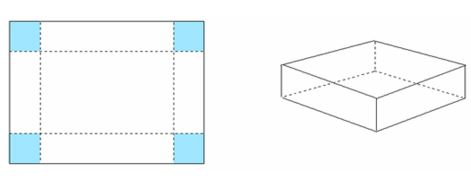
\includegraphics[width=0.5\linewidth]{images/net.png}
    \end{figure}
    Show that this is the maximum.
    \pagebreak
    \item 
    \begin{enumerate}[itemsep=6cm]
        \item 
        A car is travelling at 20 ms$^{-1}$ when the driver sees an obstruction ahead and slams on the brakes, decelerating at a rate of 2.5 ms$^{-2}$.

        How long will it take for the car to come to a complete stop? 

        \item 
        What distance will be travelled by the car before it comes to a stop?

        \item 
        If the car had less effective brakes and was only able to decelerate at 1.8 ms$^{-2}$, what is the fastest it could speed and still be able to stop in the same distance as in (b)?
    \end{enumerate}


\end{enumerate}
\pagebreak
\section*{Answers}
\begin{enumerate}[itemsep=2cm]
    \item 
    \begin{enumerate}[itemsep=2cm]
        \item Find the gradient of the curve given by $y=3x^3-x^2+7$ at the point $(2, 51)$
        
        $y'=9x^2-2x$

        $y'(2)=9(2)^2-2(2)=32$

        \item Find the x-coordinate of another point on the curve that has the same gradient as in (a).
        
        Make derivative equal to 32 and solve.

        $9x^2-2x=32$

        $x=2, -\frac{16}{9}$
    \end{enumerate}
    

    \item 
    Give the coordinates of the point on the curve $y=\frac{x^2}{2}+4x$ where the gradient is equal to 30.

    $y'=x+4$

    $x+4=30$

    $x=26$

    $y=\frac{26^2}{2}+4(26)=442$

    Coordinates are $(26,442)$


    \item 
    Find the equation of the tangent to the curve $y=5x-2x^2$ at the point where $x=3$.
    
    Find y-coordinate:

    $y=5(3)-2(3)^2=-3$

    Find gradient at $x=3$:

    $y'=5-4x$

    $y'(3)=5-4(3)=-7$

    $y=-7x+c$

    Substitute in coordinates to find c:

    $-3=-7(3)+c$

    $c=18$

    Tangent equation is $y=-7x+18$

    \item 
    Find the equation of the tangent to the curve $y=\frac{2x^3}{3}-x^2+4x-1$ at the point $(0,-1)$

    $y'=2x^2-2x+4$

    $y'(0)=4$

    $y=4x+c$

    To find c, substitute in the $x$ and $y$ coordinates:

    $-1=4(0)+c \Rightarrow c=-1$

    So the tangent equation is $y=4x-1$

    \item 
    For what values of $x$ is the function $f(x)=4x^3+2x^2-1$ decreasing?
    
    Decreasing means that the gradient is negative, so we differentiate and find when $f'(x)<0$

    $f'(x)=12x^2+4x$

    $12x^2+4x<0$

    Solving, $x=0, -\frac{1}{3}$

    Since it is a positive parabola, it will be below zero between the roots, therefore the function is decreasing when $-\frac{1}{3}<x<0$

    \item 
    The curve $f(x)=x^3+px^2-5$ has a gradient of 20 at the point where $x=2$. Find the value of $p$.

    $f'(x)=3x^2+2px$

    $3(2)^2+2p(2)=20$

    $12+4p=20$

    $4p=8$

    $p=2$

    \item 
    A piece of cardboard is 50cm x 30cm in size. If the corners are cut out as shown below, the cardboard can be folded into an open-topped box.

    Find the maximum volume of that box.

    \begin{figure}[h]
        \centering
        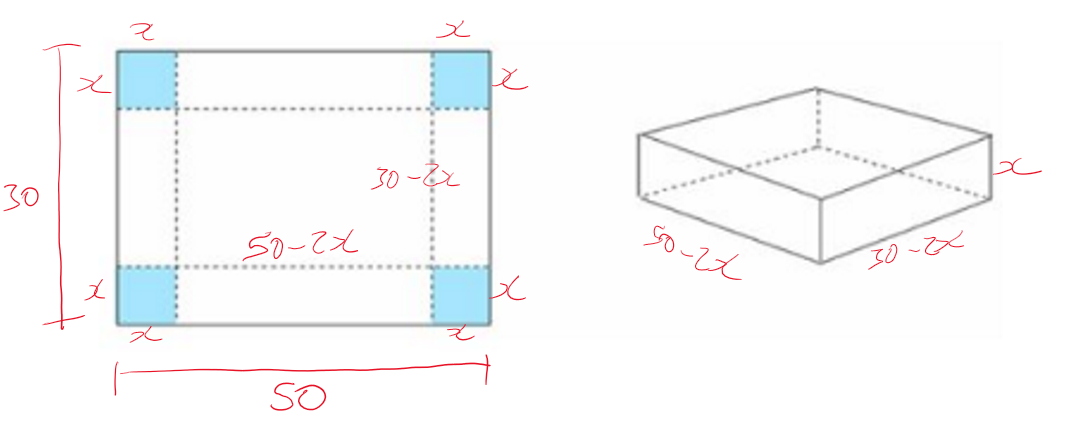
\includegraphics[width=0.5\linewidth]{images/annotated_net.png}
    \end{figure}
    Show that this is the maximum.
    
    Make $x$ the length of each cut.

    This means the base of the box is $50-2x$ wide by $30-2x$ long, and $x$ high.

    $V=x(50-2x)(30-2x)$

    $V=4x^3-160x^2+1500x$

    $V'=12x^2-320x+1500$

    $12x^2-320x+1500=0$

    $x=20.6, 6.07$

    We know $x$ can not be 20.6 as that would make one of the side lengths negative ($30-2(20.6)<0$). Therefore, $x=6.07$.

    This makes the volume $V=4(6.07)^3-160(6.07)^2+1500(6.07)=4104.4cm^2$

    To show this is a maximum we can simply say that since the volume function is a positive cubic, by the shape of the graph we know that the first turning point will be the maximum, and the second will be a minimum. 

    Or we can do the second derivative test.

    $V''=24x-320$

    $V''(6.07)=-174$

    Since the second derivative gives a negative value, the turning point must be a maximum at $x=6.07$.

    \item 
    \begin{enumerate}[itemsep=2cm]
        \item 
        A car is travelling at 20 ms$^{-1}$ when the driver sees an obstruction ahead and slams on the brakes, decelerating at a rate of 2.5 ms$^{-2}$.

        How long will it take for the car to come to a complete stop? 

        Since he decelerates at 2.5 every second, $20 \div 2.5=8$, it will take 8 seconds.

        \item 
        What distance will be travelled by the car before it comes to a stop?

        $a=-2.5$

        $v=-2.5t+c$

        Initial velocity is 20:

        $20=-2.5(0)+c \Rightarrow c=20$

        $v=-2.5t+20$

        $s=-1.25t^2+20t+C$

        Initial distance is zero, as we start measuring when the brakes are applied:

        $0=-1.25(0)^2+20(0)+C \Rightarrow C=0$

        $s=-1.25t^2+20t$

        Distance when $t=8$:

        $s=-1.25(8)^2+20(8)=80m$

        \item 
        If the car had less effective brakes and was only able to decelerate at 1.8 ms$^{-2}$, what is the fastest it could speed and still be able to stop in the same distance as in (b)?

        $a=-1.8$

        $v=-1.8t+K$ (where K is the initial velocity that we are finding)

        We first find how long it takes to stop (when velocity equals zero) in terms of K:

        $0=-1.8t+K$

        $t=\frac{K}{1.8}$

        Now we integrate $v$ to find an expression for distance, and substitute into it:

        $s=-0.9t^2+Kt$

        $80=-0.9(\frac{K}{1.8})^2+K(\frac{K}{1.8})$

        $80=-0.9\frac{K^2}{3.24}+\frac{K^2}{1.8}$

        $80=\frac{-0.9K^2}{3.24}+\frac{1.8K^2}{3.24}$

        $\frac{0.9K^2}{3.24}=80$

        $0.9K^2=259.2$

        $K^2=288$

        $K=16.97ms^{-1}$

    \end{enumerate}


\end{enumerate}
\end{document}
